%%%%%%%%%%%%%%%%%%%%%%%%%%%%%%%%%%%%%
% UI-KAPITEL
%%%%%%%%%%%%%%%%%%%%%%%%%%%%%%%%%%%%%
\chapter{Benutzeroberfläche (UI)}
\renewcommand{\authorinitials}{NK}
\label{chap:ui}

\section{Einleitung}
Die Benutzeroberfläche stellt die Verbindung zwischen Nutzer:innen und den technischen Funktionalitäten der Smart Shopping App her. Sie spielt eine zentrale Rolle bei der täglichen Nutzung der App, da sie das Hinzufügen von Produkten zur Einkaufsliste, das Anzeigen und Bearbeiten der Listen sowie die Darstellung der Preisinformationen und Marktvergleiche ermöglicht.

\section{Mockups und zentrale Ansichten}
% Hier können später Skizzen/Mobile Screenshots oder Diagramme eingefügt werden.

% Screenshots der wichtigsten UI-Zustände

% Screenshots der wichtigsten UI-Zustände nebeneinander
\begin{figure}[h!]
    \centering
    \begin{minipage}[b]{0.23\textwidth}
        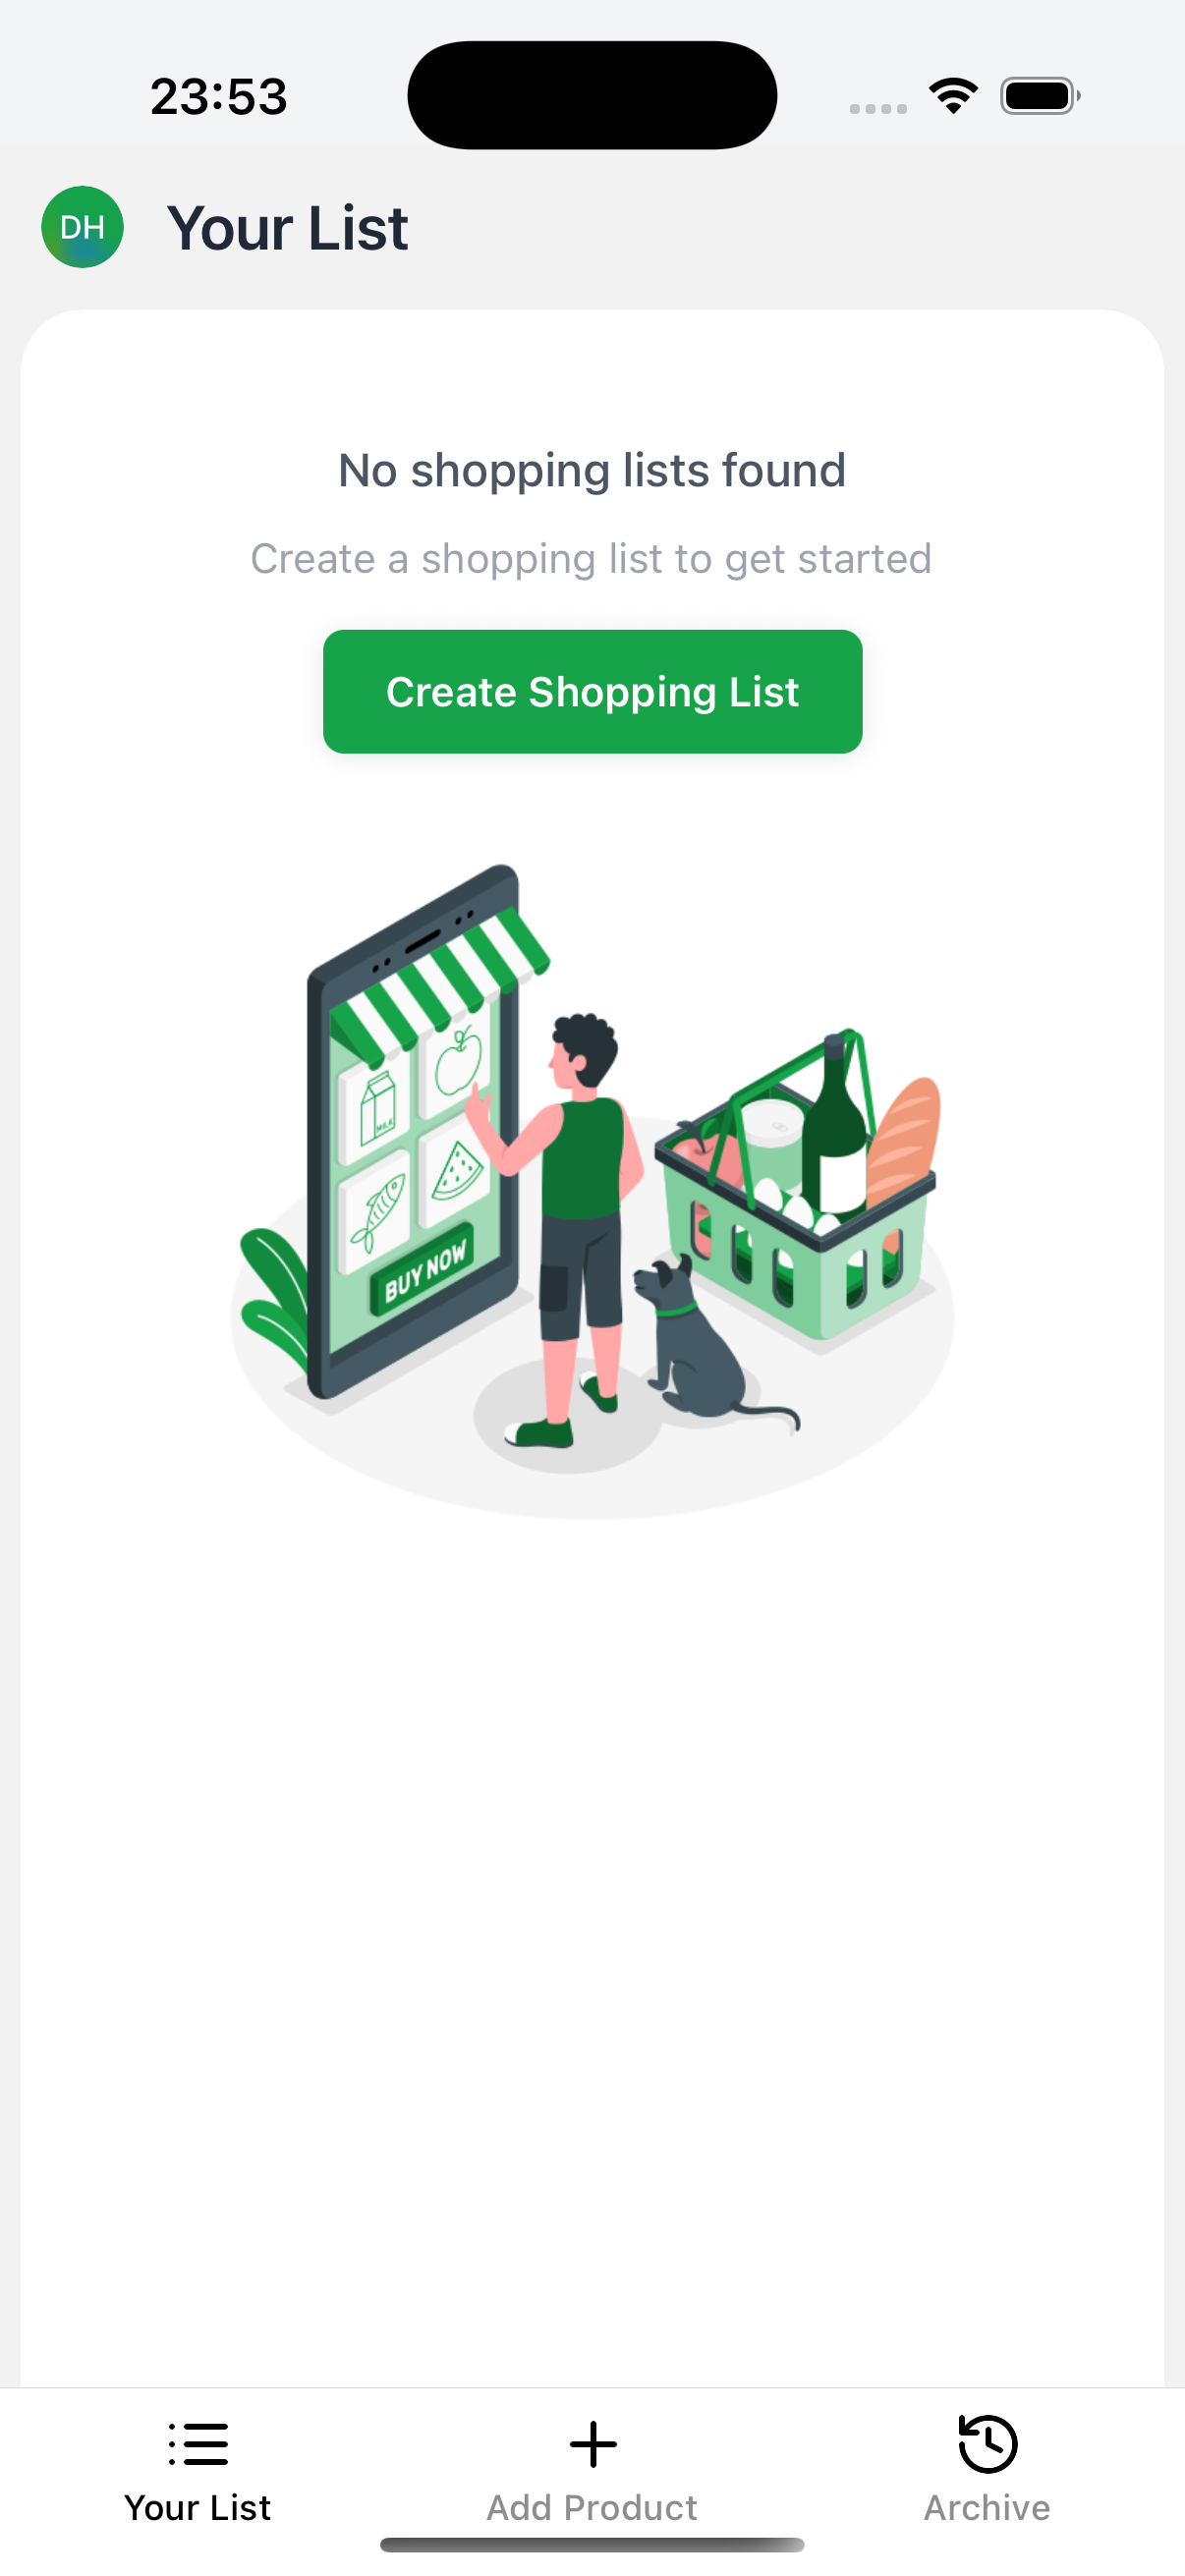
\includegraphics[width=\textwidth]{media/empty-list.png}
        \caption*{Keine Einkaufsliste}
    \end{minipage}
    \hspace{0.01\textwidth}
    \begin{minipage}[b]{0.23\textwidth}
        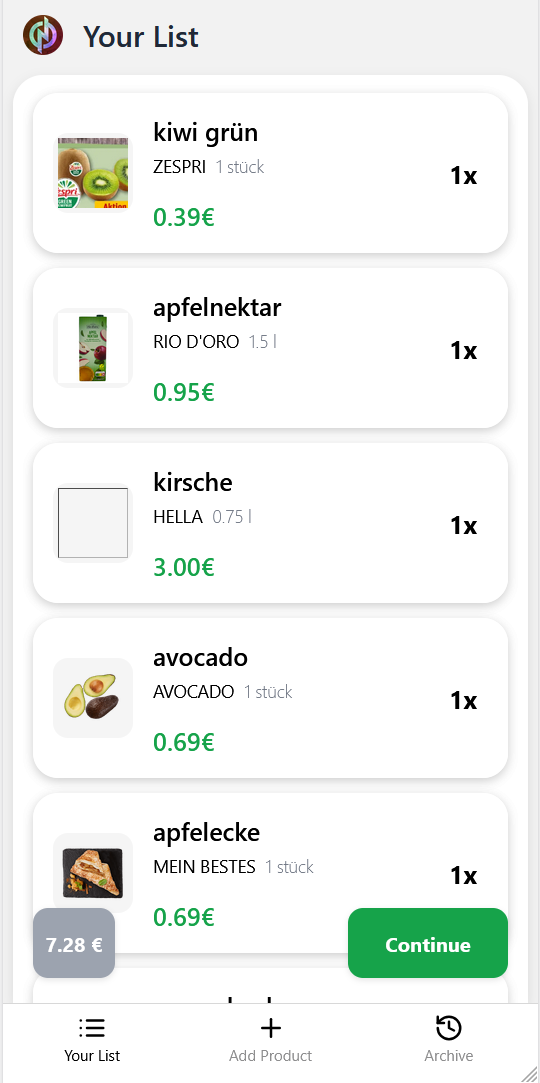
\includegraphics[width=\textwidth]{media/full-list.png}
        \caption*{Volle Einkaufsliste}
    \end{minipage}
    \hspace{0.01\textwidth}
    \begin{minipage}[b]{0.23\textwidth}
        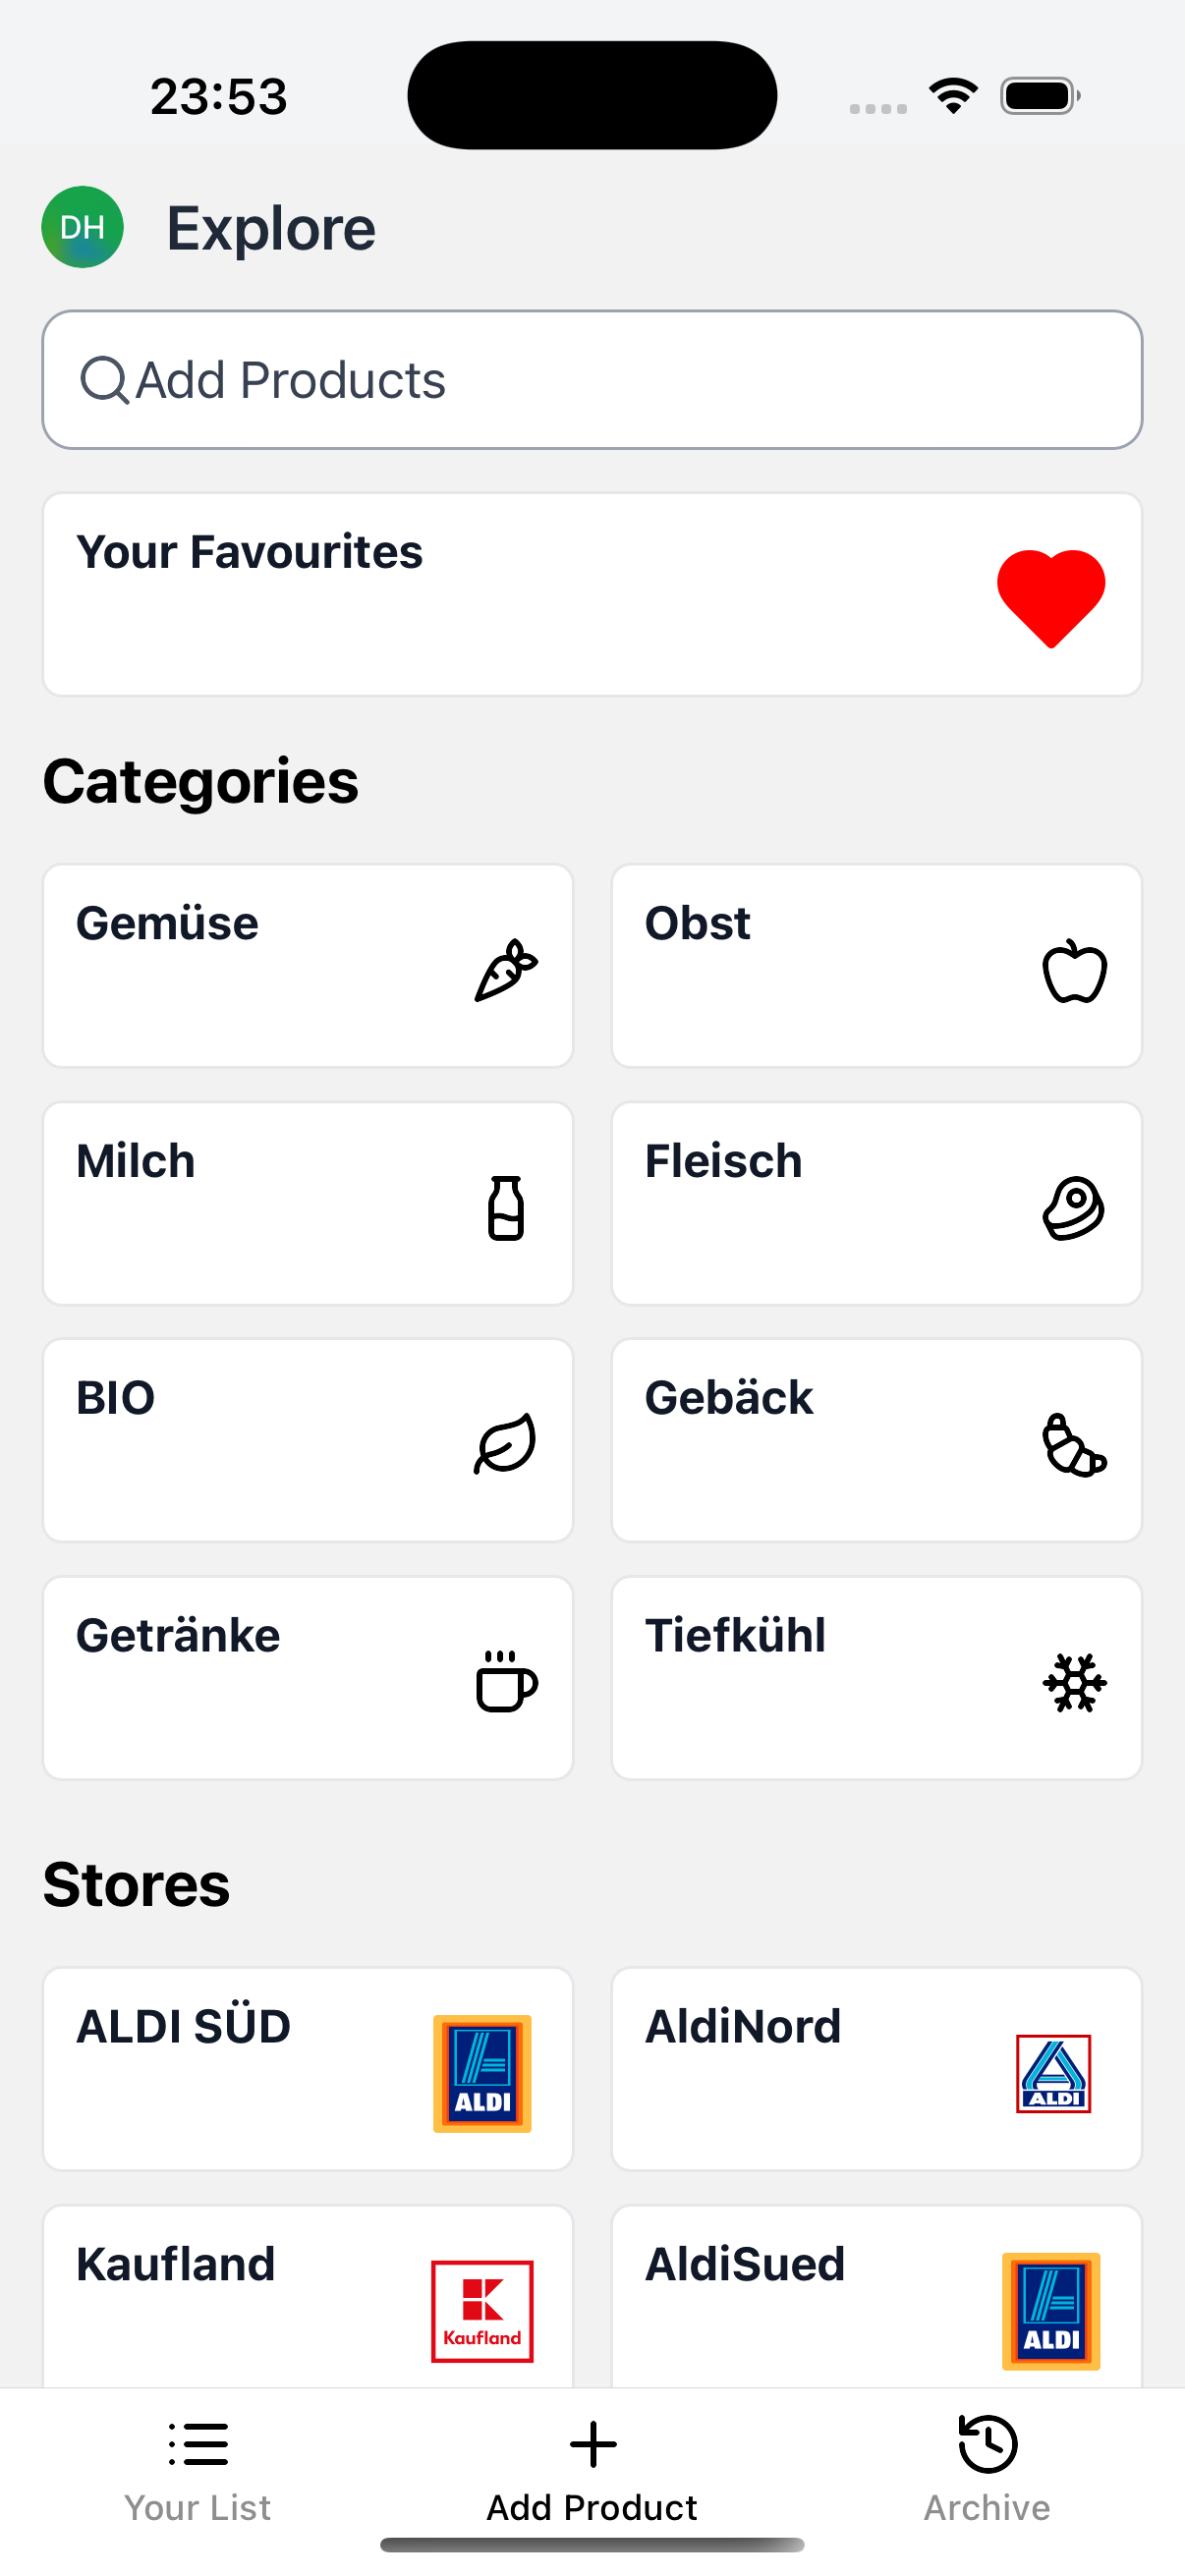
\includegraphics[width=\textwidth]{media/explore.png}
        \caption*{Explore}
    \end{minipage}
    \hspace{0.01\textwidth}
    \begin{minipage}[b]{0.23\textwidth}
        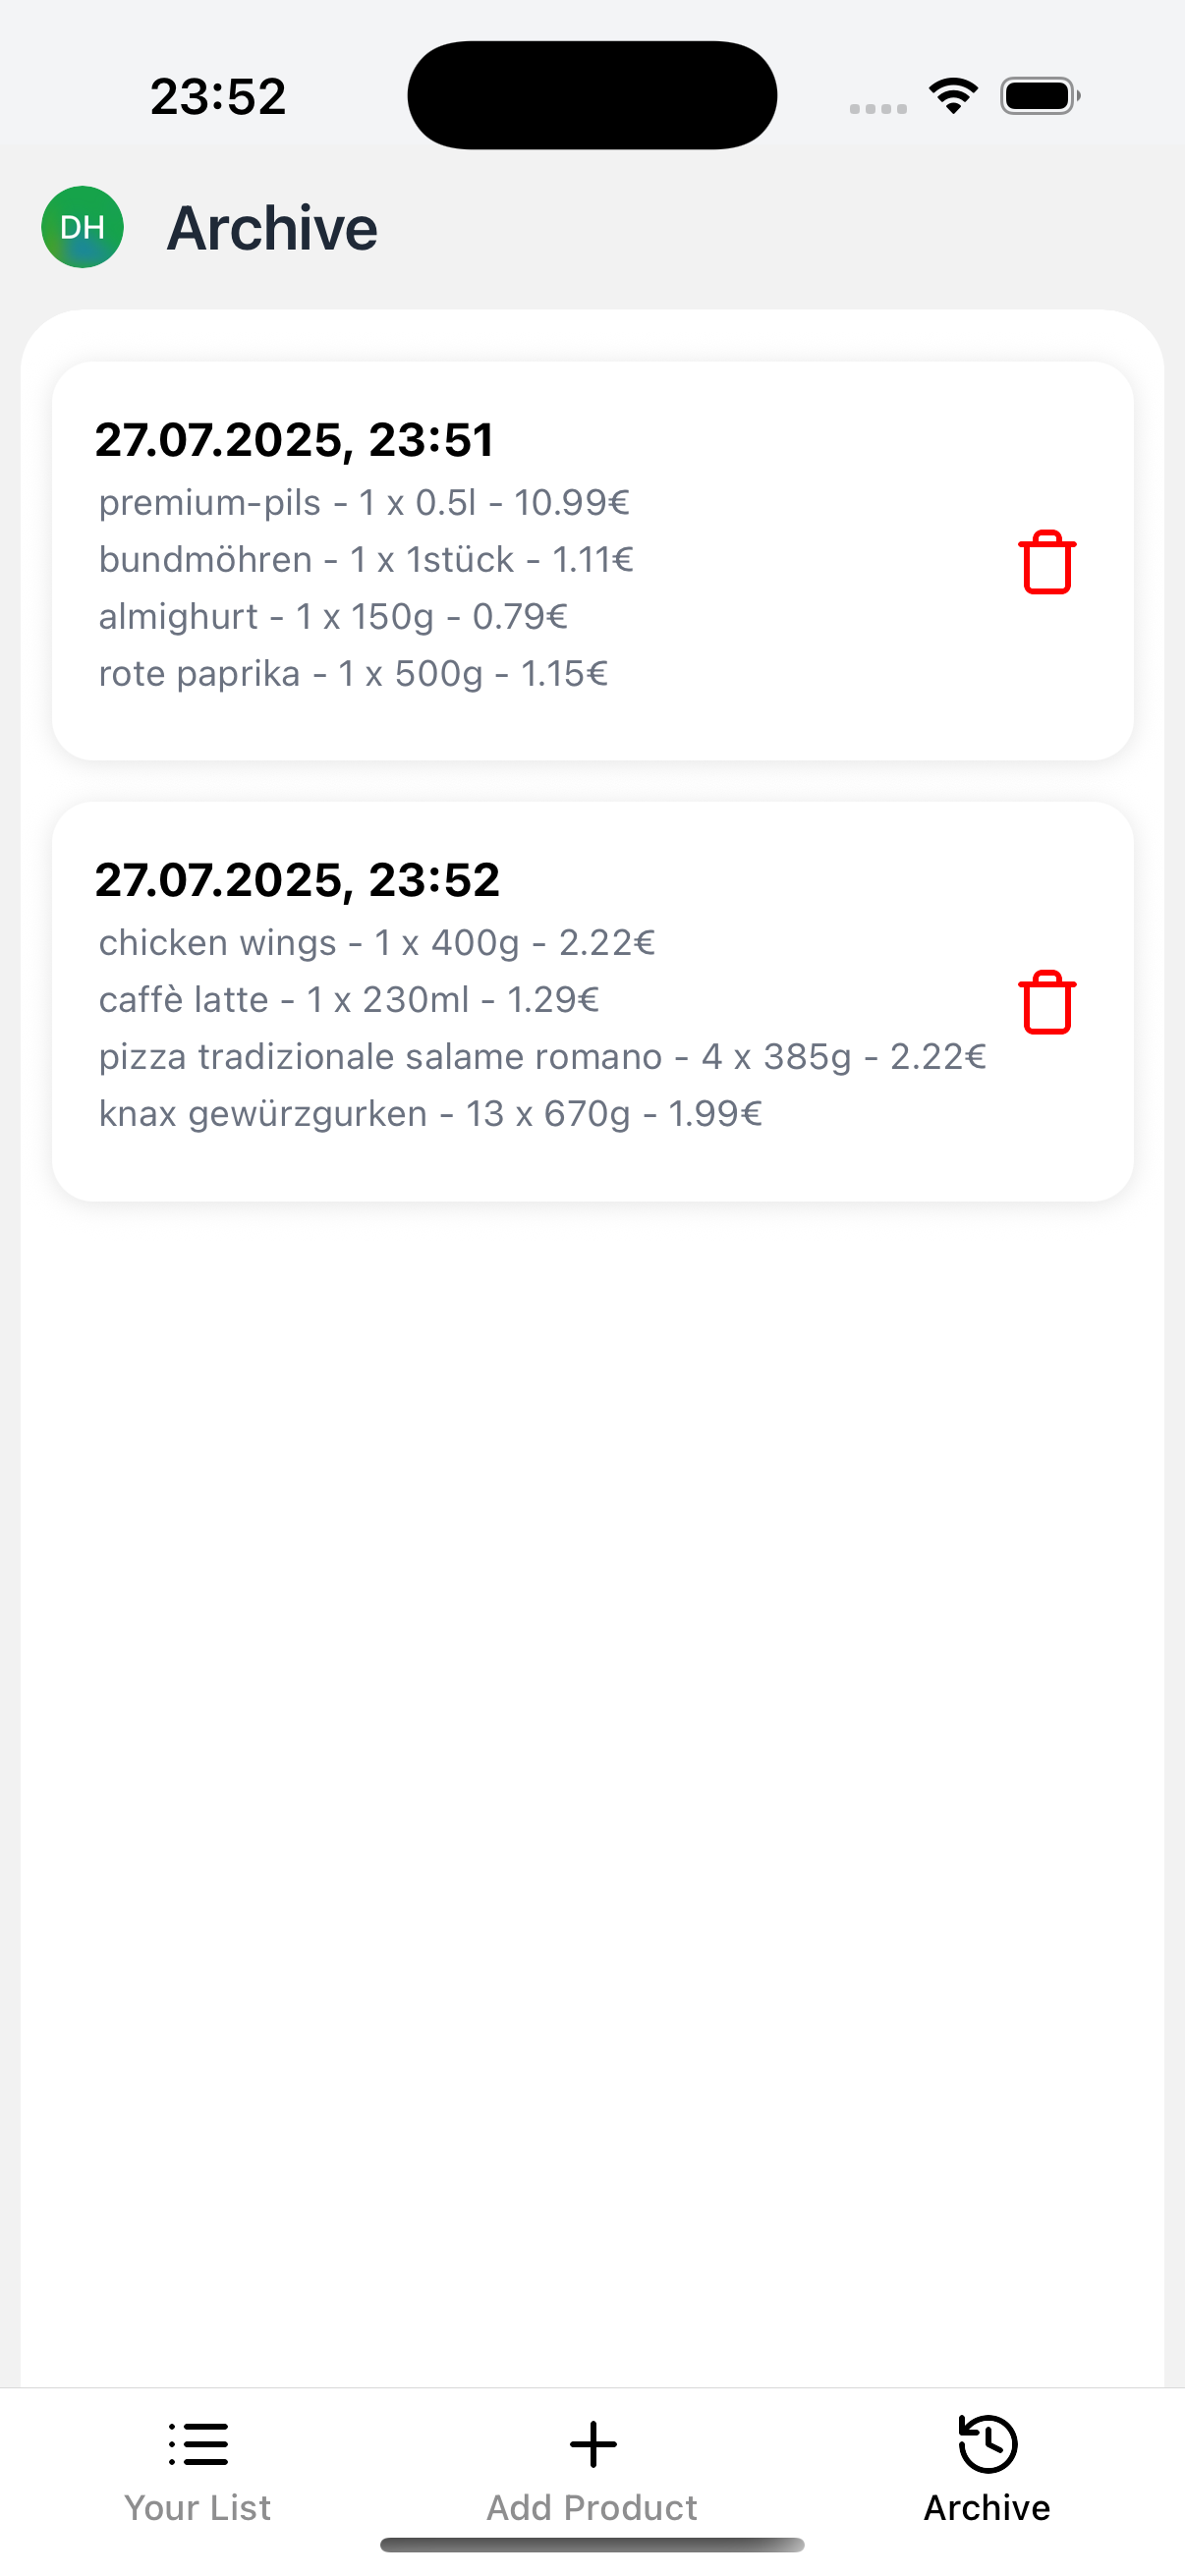
\includegraphics[width=\textwidth]{media/archive.png}
        \caption*{Archiv}
    \end{minipage}
    \caption{Wichtige UI-Zustände: Keine Liste, Explore/Add Product, Volle Liste, Archiv.}
\end{figure}

\section{Home-Screen}
\label{sec:home_screen}

\subsection{Nutzerperspektive}

\subsubsection{Zweck des Screens}
Der Home-Screen dient als zentrale Übersicht für die Einkaufsliste des Nutzers und stellt den wichtigsten Interaktionspunkt der Anwendung dar. Hier kann der Nutzer seine aktuelle Einkaufsliste einsehen und einzelne Produkte aus der Liste entfernen. Darüber hinaus besteht die Möglichkeit, die gesamte Liste zu archivieren oder eine neue Einkaufsliste anzulegen, falls noch keine existiert. Der Screen zeigt außerdem den Gesamtpreis der Liste an und ermöglicht den direkten Wechsel zur Detailansicht der Liste.

\subsubsection{UI/UX-Beschreibung}

\textbf{Wichtige UI-Elemente:}
\begin{itemize}
    \item \textbf{TopBar:} Navigationsleiste am oberen Rand
    \item \textbf{ScrollView:} Zeigt die Einkaufsliste als scrollbare Kartenansicht
    \item \textbf{Card-Komponenten:} Jede Karte repräsentiert ein Produkt mit Name, Marke, Menge, Preis, Bild und Lösch-Button
    \item \textbf{ButtonSquare:} Button zum Wechsel in die Detailansicht der Liste
    \item \textbf{Floating View:} Zeigt den Gesamtpreis der Liste an
    \item \textbf{"Create Shopping List"-Button:} Erscheint, wenn noch keine Liste existiert
\end{itemize}

\noindent\textbf{Interaktive Elemente:}
Die Benutzerinteraktion erfolgt über verschiedene gut erreichbare Elemente. Produkte können über den Lösch-Button auf jeder Produktkarte entfernt werden, während die gesamte Einkaufsliste über einen entsprechenden Button archiviert werden kann. Das Anlegen neuer Listen erfolgt über den "Create Shopping List"-Button, und der Wechsel zur Detailansicht ist über den Button mit Einkaufswagen-Icon möglich.

\subsubsection{User Flow}

\textbf{Von welchem Screen kommt der Nutzer hierher?}
Der Nutzer gelangt meistens über die Tab-Navigation als Startscreen oder nach dem Login auf den Home-Screen.

\noindent\textbf{Wohin geht es von hier aus?}
Vom Home-Screen aus stehen dem Nutzer verschiedene Navigationsmöglichkeiten zur Verfügung. Er kann zur Detailansicht der Einkaufsliste wechseln, indem er die entsprechende Option auswählt. Darüber hinaus besteht die Möglichkeit, zu Produktdetails zu navigieren, sofern diese Funktionalität über die Produktkarten implementiert ist. Weitere Optionen umfassen das Archivieren der aktuellen Liste oder das Anlegen einer neuen Liste.

\subsection{Technische Perspektive}

\subsubsection{Code-Architektur}

\textbf{Komponenten:}
\begin{itemize}
    \item ListScreen (Hauptkomponente)
    \item TopBar (Navigationsleiste)
    \item Card (Produktkarte)
    \item ButtonSquare (Floating Action Button)
    \item LoadingSpinner (Ladeanzeige)
\end{itemize}

\noindent\textbf{State Management:}
\begin{itemize}
    \item React State (useState, useEffect, useCallback)
    \item Kontext: useProductContext für Produktdaten und Ladezustand
\end{itemize}

\noindent\textbf{Services/APIs:}
Die Kommunikation mit dem Backend erfolgt über den api-Service, der alle Backend-Requests abwickelt. Dieser umfasst Funktionen wie getShoppingListItems zum Abrufen der Listenelemente, createShoppingList zum Erstellen neuer Listen, deleteFromShoppingList zum Entfernen von Produkten und archiveShoppingList zum Archivieren von Listen.

\subsubsection{Wichtige Funktionen/Methoden}
\begin{itemize}
    \item \textbf{loadList:} Lädt die aktuelle Einkaufsliste und prüft, ob eine existiert.
    \item \textbf{handleCreateShoppingList:} Erstellt eine neue Einkaufsliste via API.
    \item \textbf{handleDelete:} Löscht ein Produkt aus der Liste.
    \item \textbf{handleArchiveList:} Archiviert die aktuelle Liste.
    \item \textbf{calculateTotal:} Berechnet den Gesamtpreis der Einkaufsliste.
    \item \textbf{Scroll-Handling:} Zeigt/Versteckt Floating Buttons je nach Scrollposition (Performance-Optimierung mit react-native-reanimated).
\end{itemize}

\subsubsection{Besondere Herausforderungen}
Bei der Entwicklung des Home-Screens entstanden verschiedene technische Herausforderungen, die spezielle Lösungsansätze erforderten. Die Performance-Optimierung wurde durch den Einsatz von Reanimated für die Animation der Floating Buttons erreicht, um ein flüssiges Benutzererlebnis zu gewährleisten. Eine umfangreiche Fehlerbehandlung mit Alerts und Fallbacks stellt sicher, dass die Anwendung auch bei fehlgeschlagenen API-Requests stabil funktioniert.

Ein besonderer Fokus lag auf der User Experience, wobei unterschiedliche UI-Zustände wie das Fehlen einer Liste, eine leere Liste oder eine gefüllte Liste klar unterschieden und dem Nutzer verständlich kommuniziert werden. Die Synchronisation der Daten wird durch das automatische Neuladen der Liste bei jedem Fokus auf den Screen mittels useFocusEffect gewährleistet, sodass immer die aktuellsten Daten angezeigt werden.

\section{Explore-Screen}
\label{sec:explore_screen}

\subsection{Nutzerperspektive}

\subsubsection{Zweck des Screens}
Der Explore-Screen dient dazu, dem Nutzer eine strukturierte Übersicht über Produktkategorien und verfügbare Supermärkte zu bieten. Dieser Screen ermöglicht es dem Nutzer, gezielt nach Produkten zu suchen, verschiedene Kategorien zu durchstöbern oder Angebote von bestimmten Märkten anzeigen zu lassen. Dadurch wird eine intuitive Navigation durch das gesamte Produktsortiment der App gewährleistet.

\subsubsection{UI/UX-Beschreibung}

\textbf{Zentrale Elemente:}
\begin{itemize}
    \item Oben befindet sich eine Navigationsleiste (TopBar).
    \item Ein prominenter Button ('Add Products') ermöglicht die Produktsuche.
    \item Darunter werden die Lieblingskategorien ('Your Favourites') angezeigt.
    \item Es folgt eine Liste von Kategorien (z.B. Gemüse, Obst, Milch).
    \item Am unteren Ende werden verfügbare Stores (Supermärkte) als auswählbare Felder angezeigt, farblich hervorgehoben je nach Markt.
\end{itemize}

\noindent\textbf{Interaktive Elemente:}
Die Benutzerinteraktion erfolgt über zwei Hauptkategorien von Elementen. Der 'Add Products'-Button öffnet die Produktsuche und ermöglicht den direkten Einstieg in die Produktauswahl. Zusätzlich sind sowohl Kategorien als auch Stores als anklickbare Elemente gestaltet, die zu einer gefilterten Produktsuche führen und dem Nutzer eine zielgerichtete Navigation ermöglichen.

\subsubsection{User Flow}

\textbf{Einstieg:} Der Nutzer gelangt meist von einem Tab-Menü oder der Hauptnavigation auf diesen Screen.

\noindent\textbf{Von hier aus kann der Nutzer:}
Der Explore-Screen bietet verschiedene Navigationsmöglichkeiten für den Nutzer. Über den "Add Products"-Button kann er direkt zur Produktsuche navigieren und mit der Zusammenstellung seiner Einkaufsliste beginnen. Alternativ kann er über eine Kategorie oder einen Store gezielt Produkte filtern und anzeigen lassen, um spezifische Angebote zu finden. Nach der Auswahl wird der Nutzer zur Such- oder Produktübersicht weitergeleitet, wo er seine Auswahl verfeinern kann.

\subsection{Technische Perspektive}

\subsubsection{Code-Architektur}

\textbf{Hauptkomponente:} explore (React Functional Component)

\noindent\textbf{Eingesetzte Komponenten:}
\begin{itemize}
    \item TopBar (Navigation)
    \item SearchButton (Produktsuche)
    \item CategorieField (Favoriten)
    \item CategorieGroup (Kategorien \& Stores)
\end{itemize}

\noindent\textbf{Datenmodell:} Store-Typ aus den globalen Typen

\noindent\textbf{API:} Daten werden über api.getStores() geladen

\noindent\textbf{State Management:} React useState/useEffect (lokaler State)

\subsubsection{Wichtige Funktionen/Methoden}

\begin{itemize}
    \item \textbf{getStoreColor(name: string):} Weist jedem Store eine spezifische Farbe zu.
    \item \textbf{useEffect + fetchStores:} Lädt beim ersten Rendern die Store-Liste asynchron von der API und speichert sie im State.
    \item \textbf{Interaktive Elemente (onPress):} Navigieren mit router.push zur Suchseite, ggf. mit Store-Filter.
\end{itemize}

\subsubsection{Besondere Herausforderungen}
Die Entwicklung des Explore-Screens brachte verschiedene technische Herausforderungen mit sich. Das dynamische Laden und Anzeigen der Stores mit individueller Farbcodierung erforderte eine flexible Architektur, die eine einheitliche Darstellung bei unterschiedlichen Datenquellen gewährleistet. Eine robuste Fehlerbehandlung beim Laden der Stores wurde implementiert, die dem Nutzer mittels Alert-Nachrichten bei Problemen entsprechendes Feedback gibt. Zusätzlich stellte die Gestaltung einer übersichtlichen und intuitiven Benutzeroberfläche trotz der vielen Auswahlmöglichkeiten eine besondere Herausforderung dar, die durch eine durchdachte Kategorisierung und visuelle Hierarchie gelöst wurde.

\section{Search-Screen}
\label{sec:search_screen}

\subsection{Nutzerperspektive}

\subsubsection{Zweck des Screens}
Der Search-Screen ermöglicht es dem Nutzer, gezielt nach Produkten zu suchen, verschiedene Filter anzuwenden und gefundene Produkte zur Einkaufsliste hinzuzufügen. Das Hauptziel besteht darin, eine schnelle und komfortable Möglichkeit zu bieten, passende Angebote zu finden und die Produktauswahl durch Filter für Kategorie und Store zu verfeinern. Dieser Screen stellt somit das Herzstück der Produktsuche und -auswahl dar.

\subsubsection{UI/UX-Beschreibung}

\textbf{Zentrale Elemente:}
\begin{itemize}
    \item \textbf{Suchleiste:} Oben mittig, ermöglicht die Suche nach Produktnamen oder Marken.
    \item \textbf{Filter-Button:} Links neben der Suchleiste öffnet ein Modal für Filteroptionen (Kategorie, Store).
    \item \textbf{Cancel-Button:} Rechts neben der Suchleiste, löscht die aktuelle Suche.
    \item \textbf{Produktliste:} Zeigt gefilterte oder alle Produkte als Karten an, sortiert nach günstigstem Preis.
    \item \textbf{Produktkarte:} Enthält Produktdetails und einen Button (PlusCircle), um das Produkt zur Einkaufsliste hinzuzufügen.
    \item \textbf{Filter-Modal:} Ermöglicht Mehrfachauswahl von Kategorien und Stores, sowie das Zurücksetzen oder Anwenden der Filter.
    \item \textbf{Ladespinner:} Wird angezeigt, solange die Produktdaten geladen werden.
\end{itemize}

\noindent\textbf{Interaktive Elemente:}
Der Search-Screen bietet dem Nutzer verschiedene Interaktionsmöglichkeiten für eine effiziente Produktsuche. Die Suchleiste als Textinput ermöglicht die direkte Eingabe von Suchbegriffen, während der Filter-Button ein Modal mit erweiterten Filteroptionen öffnet. Ein Cancel-Button setzt die aktuelle Suche zurück und ermöglicht einen Neustart. Die Produktkarten sind klickbar und führen zur Detailansicht der jeweiligen Artikel. Der PlusCircle-Button auf jeder Karte fügt das entsprechende Produkt direkt zur Einkaufsliste hinzu. Das Filter-Modal selbst enthält MultiSelects für die Auswahl sowie Reset- und Apply-Buttons für die Filterverwaltung.

\subsubsection{User Flow}
\textbf{Einstieg:} Der Nutzer gelangt meist von einem Tab oder durch Auswahl eines Stores auf den Search-Screen.

\noindent\textbf{Aktionen:} Auf diesem Screen kann der Nutzer verschiedene Aktionen durchführen, um seine Produktsuche zu optimieren. Er kann gezielt nach Produkten suchen, verschiedene Filter anwenden, gefundene Produkte direkt zur Einkaufsliste hinzufügen oder detaillierte Produktinformationen aufrufen.

\noindent\textbf{Navigation:}
Die Navigation vom Search-Screen aus bietet verschiedene Möglichkeiten. Ein Klick auf ein Produkt führt zur Detailansicht, während das Anwenden von Filtern eine aktualisierte Produktliste zur Verfügung stellt. Darüber hinaus ist die Rückkehr zu anderen Tabs oder Screens jederzeit möglich, um einen flexiblen Workflow zu gewährleisten.

\subsection{Technische Perspektive}

\subsubsection{Code-Architektur}

\textbf{Hauptkomponente:} SearchSite (funktionale React-Komponente)

\noindent\textbf{Verwendete Komponenten:}
\begin{itemize}
    \item SearchBar (benutzerdefinierte Suchleiste)
    \item CustomMultiSelect (Filterauswahl)
    \item SearchCard (Produktkarte)
    \item ButtonSizeable, ButtonTransparent (Buttons)
    \item LoadingSpinner (Ladesymbol)
\end{itemize}

\noindent\textbf{State Management:} React Context (useProductContext) für Produkte und Laden-Status

\noindent\textbf{API:} Zugriff auf Stores und Produkte über api-Service

\subsubsection{Abhängigkeiten}

\textbf{Services:} api (z.B. getStores, addToShoppingList)

\noindent\textbf{State:} Produkte, Stores, Filterauswahl, Suchbegriff, Ladezustand

\noindent\textbf{Libraries:} expo-router, @shopify/flash-list, lucide-react-native (Icons), React Native Komponenten

\subsubsection{Wichtige Funktionen/Methoden}
\begin{itemize}
    \item \textbf{handleSearch(query):} Filtert Produkte nach Suchbegriff und sortiert nach Preis.
    \item \textbf{applyFilters():} Wendet Suchbegriff, Kategorie- und Store-Filter an, sortiert Ergebnis.
    \item \textbf{fetchStores():} Holt Store-Daten von der API.
    \item \textbf{useEffect-Hooks:}
    \begin{itemize}
        \item Lädt Stores beim Mounten.
        \item Setzt Store-Filter, wenn ein Store-Name als Parameter übergeben wird.
        \item Lädt Produkte, falls noch nicht vorhanden.
        \item Wendet Filter automatisch an, wenn sich die Store-Auswahl ändert.
    \end{itemize}
    \item \textbf{renderItem:} Rendert einzelne Produktkarten mit Interaktionsmöglichkeiten.
\end{itemize}

\subsubsection{Besondere Herausforderungen}
Die Entwicklung des Search-Screens stellte verschiedene komplexe Herausforderungen dar, die innovative Lösungsansätze erforderten. Die Implementierung der Filterlogik erwies sich als besonders anspruchsvoll, da eine Kombination aus Suchbegriff, Kategorie- und Store-Filter inklusive intelligenter Sortierung realisiert werden musste. Für die Performance-Optimierung wurde FlashList eingesetzt, um auch bei großen Produktlisten ein performantes Rendering zu gewährleisten.

Die State-Synchronisation stellte eine weitere Herausforderung dar, da Filter automatisch bei Änderung der Auswahl angewendet und gleichzeitig mit dem globalen Context synchronisiert werden müssen. Besondere Aufmerksamkeit galt auch der User Experience, wobei eine durchdachte Reset- und Apply-Logik im Filter-Modal implementiert wurde, die dem Nutzer sofortige Rückmeldung bei Suche und Filterung bietet.

\section{UI-Komponenten}
\label{sec:ui_komponenten}

\subsection{Home(index)}

\subsubsection{Card}

\noindent\textbf{Aufbau und Funktionsweise:}
Die Card-Komponente ist eine React Native-Komponente, die die Daten eines einzelnen Produkts als Karte darstellt. Sie erhält alle relevanten Produktinformationen (Name, Marke, Größe, Einheit, Preis, Menge, Bild-URL) sowie optionale Callback-Funktionen für das Auswählen (onPress) und Löschen (onDelete). Die Komponente nutzt einen Swipeable-Container, um die Löschfunktion per Wischgeste zu ermöglichen.

\noindent\textbf{Darstellung:}
Das Produkt wird in einer horizontalen Karte angezeigt. Links befindet sich das Produktbild, daneben die Produktdetails wie Name, Marke, Größe, Einheit und Preis. Die Menge wird, falls vorhanden, ganz rechts angezeigt. Die Karte ist optisch ansprechend gestaltet, mit abgerundeten Ecken, Schatten und modernen Farben.

\noindent\textbf{Interaktive Elemente:}
Die Karte kann angetippt werden, um eine Aktion auszulösen (z.\,B. Details anzeigen), sofern eine onPress-Funktion übergeben wurde. Durch Wischen nach links erscheint ein rotes Feld mit einem Papierkorb-Icon, über das das Produkt gelöscht werden kann. Die Löschfunktion wird nur angezeigt, wenn eine onDelete-Funktion vorhanden ist.

\noindent\textbf{Verwendung:}
Die Card-Komponente wird innerhalb von Produktlisten eingesetzt, um einzelne Produkte übersichtlich und interaktiv darzustellen. Sie eignet sich besonders für Einkaufslisten oder Produktübersichten, bei denen Nutzer Produkte auswählen oder entfernen können. Die Komponente ist flexibel und kann in verschiedenen Kontexten wiederverwendet werden.

\subsection{Explore}

\subsubsection{CategorieField}
Die Komponente CategorieField ist ein wiederverwendbares React Native-UI-Element, das eine Kategorie als anklickbares Feld darstellt. Sie nimmt folgende Props entgegen:
\begin{itemize}
    \item \textbf{title:} Der Name der Kategorie (wird als Text angezeigt).
    \item \textbf{image:} Optionales Bild, das dekorativ rechts oben im Feld angezeigt wird.
    \item \textbf{backgroundColor:} Optionaler Hintergrundfarbwert (Standard: "\#4B946A").
    \item \textbf{onPress:} Optionaler Callback, der beim Antippen des Feldes ausgeführt wird.
\end{itemize}

\noindent\textbf{Aufbau:}
Das Haupt-Element basiert auf einem Pressable, das das gesamte Feld anklickbar macht und eine intuitive Benutzerinteraktion ermöglicht. Im Feld wird der Titel als weißer, fetter Text oben links angezeigt, was eine gute Lesbarkeit gewährleistet. Falls ein Bild übergeben wird, erscheint es dekorativ rechts oben, leicht gedreht und abgerundet, was dem Design eine moderne Note verleiht. Das Layout nutzt Tailwind-Klassen und Style-Props für ein responsives und modernes Design, das sich an verschiedene Bildschirmgrößen anpasst.

\noindent\textbf{Verwendung:} Die Komponente eignet sich hervorragend, um Kategorien in einer Übersicht darzustellen, beispielsweise in einer Liste oder einem Grid-Layout. Sie kann individuell mit Titel, Bild und Farbe angepasst und mit einer spezifischen Aktion beim Klick versehen werden, was eine hohe Flexibilität in der Anwendung ermöglicht.

\subsubsection{CategorieGroup}
Die Komponente CategorieGroup dient dazu, eine Gruppe von Kategorien als übersichtliche, responsive Felder darzustellen. Sie nimmt ein Array von Kategorien entgegen und ordnet diese in Reihen mit jeweils zwei Feldern an. Bei einer ungeraden Anzahl wird das erste Feld einzeln in einer eigenen Reihe angezeigt.

\noindent\textbf{Aufbau und Funktionsweise:}

\textbf{Props:}
\begin{itemize}
    \item \textbf{categories:} Ein Array von Kategorie-Objekten mit Titel, Bild, Hintergrundfarbe und -optionaler Aktion.
    \item \textbf{onPress:} Optionaler Callback, der beim Klick auf ein Feld ausgeführt wird und die jeweilige Kategorie übergibt.
\end{itemize}

\textbf{Logik:}
Die Komponente führt zunächst eine Überprüfung durch, ob Kategorien vorhanden sind, bevor sie mit der Darstellung beginnt. Bei einer ungeraden Anzahl von Kategorien wird das erste Element einzeln angezeigt, während die restlichen Kategorien paarweise gruppiert werden. Jede Reihe wird als View mit zwei Feldern (CategorieField) dargestellt, wobei unvollständige Reihen mit einem leeren Feld aufgefüllt werden, um ein konsistentes Layout zu gewährleisten.

\textbf{Layout:}
Das Design nutzt Flexbox und Tailwind-Klassen für ein modernes, flexibles Layout, das sich verschiedenen Bildschirmgrößen anpasst. Die Felder sind gleichmäßig verteilt und haben definierte Abstände zwischen den Reihen, was eine ansprechende visuelle Hierarchie schafft.

\noindent\textbf{Verwendung:} CategorieGroup eignet sich optimal, um Kategorien in einer übersichtlichen, klickbaren Grid-Ansicht darzustellen, beispielsweise auf einer Explore-Seite. Die Komponente ist flexibel gestaltet und kann individuell mit verschiedenen Aktionen und Design-Optionen erweitert werden, um spezifische Anforderungen zu erfüllen.

\subsubsection{SearchButton}
Die Komponente SearchButton ist ein klickbarer Button, der wie ein Suchfeld aussieht, aber kein Eingabefeld ist. Sie zeigt ein Lupen-Icon und einen beschrifteten Text (Standard: "Add Products") an.

\noindent\textbf{Aufbau:}

\textbf{Props:}
\begin{itemize}
    \item \textbf{label:} Optionaler Text, der im Button angezeigt wird.
    \item \textbf{onPress:} Optionaler Callback, der beim Klick ausgeführt wird.
\end{itemize}

\textbf{Darstellung:}
Die Komponente basiert auf einem Pressable mit abgerundeten Ecken, weißem Hintergrund und grauem Rahmen, was ihr ein sauberes und professionelles Aussehen verleiht. Das Lupen-Icon (Search aus lucide-react-native) wird links neben dem Text positioniert und signalisiert dem Nutzer die Suchfunktionalität. Der Button reagiert visuell auf Berührungen durch eine verringerte Opazität und bietet auf Android-Geräten zusätzlich einen Ripple-Effekt für taktiles Feedback.

\noindent\textbf{Verwendung:} SearchButton eignet sich hervorragend als auffälliger, interaktiver Button für Such- oder Hinzufügen-Aktionen, beispielsweise am oberen Rand einer Produktliste. Die Komponente ist einfach anpassbar und kann flexibel überall eingesetzt werden, wo ein solcher funktionaler Button benötigt wird.

\subsubsection{StoreIcons}
Der Ordner icons innerhalb von categories enthält die grafischen Symbole für verschiedene Supermärkte und Einkaufskategorien, die in der App verwendet werden. Jede Icon-Komponente repräsentiert einen bestimmten Markt, wie zum Beispiel Lidl, Aldi oder Rewe, und liegt als eigene Datei im Ordner vor.

Die Datei index.tsx dient als zentrale Sammelstelle für alle Icons. Sie exportiert die einzelnen Komponenten unter einheitlichen Namen, sodass sie in anderen Teilen der Anwendung unkompliziert und übersichtlich importiert werden können. Das erleichtert die Wiederverwendung und sorgt für eine klare Struktur im Code.

Insgesamt ermöglicht dieser Aufbau, dass die Icons konsistent und effizient im Frontend eingesetzt werden können, zum Beispiel zur Visualisierung von Märkten in Listen oder Übersichten. Die zentrale Exportdatei vereinfacht die Verwaltung und trägt zur besseren Wartbarkeit des Projekts bei.

\subsection{Search}

\subsubsection{SearchBar}
Die Komponente SearchBar ist eine interaktive Suchleiste für React Native, die Benutzereingaben entgegennimmt und Suchanfragen auslöst.

\noindent\textbf{Aufbau und Funktionsweise:}

\textbf{Props:}
\begin{itemize}
    \item \textbf{placeholder:} Optionaler Platzhaltertext im Eingabefeld (Standard: "Search...").
    \item \textbf{onSearch:} Callback, der bei jeder Änderung des Suchbegriffs aufgerufen wird.
\end{itemize}

\hangindent=2em
\hangafter=1
\textbf{Ref-API:}
Über das ref kann die Methode clear von außen aufgerufen werden, um das Suchfeld zu leeren und die Tastatur zu schließen.

\textbf{Logik:}
Die Eingabe wird im State query gespeichert und jede Änderung im Textfeld löst den onSearch-Callback mit dem aktuellen Wert aus. Ein Klick auf die Leiste fokussiert das Eingabefeld automatisch, was die Benutzerfreundlichkeit erhöht. Die Methode clearSearch setzt das Feld zurück und schließt die Tastatur, um eine saubere Benutzeroberfläche zu gewährleisten.

\textbf{Darstellung:}
Die Suchleiste besteht aus einem weißen, abgerundeten Container mit einem integrierten TextInput. Das TextInput ist direkt fokussierbar und optisch schlicht gehalten, um die Aufmerksamkeit auf die Eingabe zu lenken.

\noindent\textbf{Verwendung:} SearchBar eignet sich optimal für Suchfunktionen in Listen oder Übersichten. Sie kann von außen gesteuert werden, beispielsweise zum programmatischen Zurücksetzen, und ist flexibel für verschiedene Anwendungsfälle einsetzbar.

\subsubsection{CustomMultiSelect}
Die Komponente CustomMultiSelect ist ein individuell gestaltetes Mehrfach-Auswahlfeld für React Native, basierend auf react-native-element-dropdown. Sie ermöglicht die Auswahl mehrerer Optionen aus einer Liste und bietet eine Suchfunktion.

\noindent\textbf{Aufbau und Funktionsweise:}

\textbf{Props:}
\begin{itemize}
    \item \textbf{data:} Array von Auswahloptionen mit label und value.
    \item \textbf{labelField, valueField:} Feldnamen für Anzeige und Wert.
    \item \textbf{placeholder:} Platzhaltertext im Auswahlfeld.
    \item \textbf{value:} Array der aktuell ausgewählten Werte.
    \item \textbf{onChange:} Callback, der bei Änderung der Auswahl ausgelöst wird.
    \item Diverse Style-Props zur Anpassung des Designs.
    \item \textbf{search:} Aktiviert die Suchfunktion (Standard: true).
    \item \textbf{maxHeight:} Maximale Höhe der Dropdown-Liste.
\end{itemize}

\textbf{Darstellung:}
Die Dropdown-Liste zeigt alle verfügbaren Optionen übersichtlich an, wobei ausgewählte Elemente mit einem Haken-Icon markiert werden. Ausgewählte Items werden als Chips oberhalb der Liste angezeigt und bieten die Möglichkeit zum schnellen Entfernen über ein ×-Symbol. Die Komponente ist optisch anpassbar und nutzt Tailwind-Klassen für ein modernes Design, das sich harmonisch in verschiedene UI-Kontexte einfügt.

\textbf{Logik:}
Die Auswahl und das Entfernen von Items werden vollständig über die Props gesteuert, was eine saubere Datenhaltung gewährleistet. Die integrierte Suchfunktion filtert die angezeigten Optionen in Echtzeit und verbessert die Benutzerfreundlichkeit bei großen Datensätzen.

\noindent\textbf{Verwendung:} CustomMultiSelect eignet sich hervorragend für Filter- und Auswahlfunktionen, bei denen mehrere Werte gleichzeitig gewählt werden können, beispielsweise zur Produktsuche oder Kategoriefilterung. Sie ist flexibel gestaltet und lässt sich einfach in verschiedene UI-Kontexte integrieren.

\subsection{(Produkt-)Details}

\subsubsection{Field}
Die Komponente Field ist ein flexibler, klickbarer Button für React Native, der ein Icon und optional einen Text anzeigt.

\noindent\textbf{Aufbau und Funktionsweise:}

\textbf{Props:}
\begin{itemize}
    \item \textbf{icon:} Das anzuzeigende Icon (React-Komponente).
    \item \textbf{text:} Optionaler Text, der neben dem Icon angezeigt wird.
    \item \textbf{iconColor:} Farbe des Icons (wird über das Icon selbst gesteuert).
    \item \textbf{backgroundColor:} Hintergrundfarbe des Buttons.
    \item \textbf{onPress:} Optionaler Callback, der beim Klick ausgeführt wird.
\end{itemize}

\textbf{Darstellung:}
Der Button präsentiert sich mit abgerundeten Ecken und ist horizontal ausgerichtet und zentriert angeordnet. Das Icon wird links positioniert, während der Text, falls vorhanden, rechts daneben platziert wird. Der Hintergrund ist individuell anpassbar, was eine flexible Gestaltung ermöglicht. Die Klick-Animation wird über activeOpacity gesteuert und bietet dem Nutzer visuelles Feedback bei der Interaktion.

\noindent\textbf{Verwendung:} Field eignet sich für verschiedene Interaktionsmöglichkeiten, beispielsweise als Mengen-Auswahl, Aktions-Button oder für Eingabefelder mit Icon-Unterstützung. Das Design ist flexibel angelegt und kann mit unterschiedlichen Icons, Farben und Texten verwendet werden, um verschiedene Anwendungsfälle abzudecken.

\subsubsection{QuantityInput}
Die Komponente QuantityInput ist ein Eingabefeld für Mengenangaben, das Benutzern ermöglicht, eine Zahl durch Plus- und Minus-Buttons zu erhöhen oder zu verringern.

\noindent\textbf{Aufbau und Funktionsweise:}

\textbf{Props:}
\begin{itemize}
    \item \textbf{value:} Startwert der Menge (Standard: 1).
    \item \textbf{onChange:} Callback, der bei jeder Änderung der Menge ausgelöst wird.
    \item \textbf{min, max:} Minimale und maximale erlaubte Werte (Standard: 1 bis 99).
\end{itemize}

\textbf{Logik:}
Die aktuelle Menge wird im State quantity verwaltet und bietet eine zentrale Kontrolle über den Wert. Beim Klick auf den Minus-Button wird die Menge um eins verringert, solange sie über dem definierten Minimum liegt. Entsprechend wird beim Klick auf den Plus-Button die Menge um eins erhöht, solange sie unter dem festgelegten Maximum bleibt. Jede Änderung löst den onChange-Callback mit dem neuen Wert aus, was eine nahtlose Integration in übergeordnete Komponenten ermöglicht.

\textbf{Darstellung:}
Die Komponente besteht aus einer horizontal angeordneten Reihe mit einem Minus-Button, der zentralen Mengenanzeige und einem Plus-Button. Die Buttons sind rund gestaltet und heben sich optisch deutlich ab, während die aktuelle Menge mittig und gut lesbar angezeigt wird.

\noindent\textbf{Verwendung:} QuantityInput eignet sich optimal für Produktdetailseiten oder Warenkörbe, wo Nutzer die gewünschte Menge eines Artikels präzise einstellen können. Sie ist intuitiv bedienbar und flexibel in verschiedenen Kontexten einsetzbar.

\subsubsection{ProductLoadingSkeleton}
Die Komponente ProductLoadingSkeleton zeigt ein Ladeplatzhalter-Layout für Produktdetailseiten an, während die echten Daten geladen werden.

\noindent\textbf{Aufbau und Funktionsweise:}

\textbf{Darstellung:}
Die Komponente besteht aus mehreren grauen, animierten Rechtecken (``Skeletons''), die die Struktur der später angezeigten Produktinformationen nachahmen und dem Nutzer eine Vorschau auf das kommende Layout bieten. Es sind Platzhalter für das Produktbild, den Titel, Varianten, Angebote und einen Button vorhanden, die alle wichtigen Bereiche der Produktdetailseite abdecken. Die Platzhalter sind mit der Klasse animate-pulse versehen, um eine pulsierende Ladeanimation darzustellen, die Aktivität signalisiert und die Wartezeit angenehmer gestaltet.

\textbf{Layout:}
Die Elemente sind optisch so angeordnet, wie die echten Produktdetails später erscheinen werden, was eine nahtlose Transition gewährleistet. Das Layout ist responsiv gestaltet und zentriert ausgerichtet, um auf verschiedenen Bildschirmgrößen optimal zu funktionieren.

\noindent\textbf{Verwendung:} ProductLoadingSkeleton wird angezeigt, wenn Produktdaten noch nicht vollständig geladen sind, um dem Nutzer visuelles Feedback zu geben und die Wartezeit angenehmer zu gestalten. Sie verbessert die User Experience erheblich durch ein modernes Lade-Design, das Transparenz über den Ladezustand schafft und die wahrgenommene Ladezeit reduziert.

\subsection{Generelle UI-Komponenten}

\subsubsection{NavigationBar(TopBar)}
Die TopBar-Komponente stellt die obere Navigationsleiste der App dar und sorgt für eine konsistente Benutzerführung. Sie nimmt optional einen Titel und die Information entgegen, ob ein Zurück-Button angezeigt werden soll. Ist der Zurück-Button aktiv, kann der Nutzer zur vorherigen Seite zurückkehren. Andernfalls wird das Profilbild des aktuell angemeldeten Nutzers angezeigt, das als Button dient und beim Antippen zu den Einstellungen weiterleitet. Die Komponente verwendet React Native-Elemente für das Layout und Styling sowie Expo Router für die Navigation. Die Benutzerinformationen werden über Clerk eingebunden, sodass das Profilbild dynamisch geladen wird. Das Design ist flexibel und passt sich je nach Kontext an, wodurch die Komponente universell auf verschiedenen Screens eingesetzt werden kann.

\subsubsection{SignOutButton}

\noindent\textbf{Aufbau und Funktionsweise:}
Die SignOutButton-Komponente ist eine React Native-Komponente, die die Abmeldung eines Nutzers aus der App ermöglicht. Sie verwendet das Clerk-Auth-System und ruft beim Klick auf den Button die signOut-Funktion auf. Nach erfolgreichem Logout wird der Nutzer automatisch zur Startseite weitergeleitet. Fehler beim Abmelden werden in der Konsole ausgegeben.

\noindent\textbf{Darstellung:}
Der Button ist horizontal aufgebaut und besteht aus einem roten Logout-Icon sowie dem Text \enquote{Sign out}. Das Design ist modern und passt sich je nach Plattform (iOS oder Android) an, um ein natives Erscheinungsbild zu gewährleisten. Die Farben und abgerundeten Ecken sorgen für eine klare visuelle Trennung.

\noindent\textbf{Interaktive Elemente:}
Das zentrale interaktive Element ist der Button selbst. Ein Klick darauf löst die Abmeldefunktion aus. Die Komponente reagiert auf Touch-Events und gibt visuelles Feedback durch die Gestaltung und Animationen.

\noindent\textbf{Verwendung:}
Die SignOutButton-Komponente wird überall dort eingesetzt, wo Nutzer die Möglichkeit haben sollen, sich aus der App abzumelden, beispielsweise im Profil- oder Einstellungsbereich. Sie sorgt für eine einfache und sichere Abmeldung und kann flexibel in verschiedenen Bereichen der App eingebunden werden.

\subsubsection{ButtonSquare}

\noindent\textbf{Aufbau und Funktionsweise:}
Die ButtonSquare-Komponente ist eine wiederverwendbare Schaltfläche in quadratischer Form für React Native. Sie nimmt optionale Props entgegen: eine Callback-Funktion für das Drücken (onPress), ein Icon, einen Text, zusätzliche Klassen für das Styling (className) und eine Icon-Farbe. Das Icon wird dynamisch eingefärbt und in die Schaltfläche eingefügt.

\noindent\textbf{Darstellung:}
Die Schaltfläche ist quadratisch, hat abgerundete Ecken und einen hellgrauen Hintergrund. Sie ist zentriert, leicht gepolstert und mit einem Schatten versehen, um sich optisch vom Hintergrund abzuheben. Das Icon steht im Mittelpunkt der Schaltfläche und kann farblich angepasst werden.

\noindent\textbf{Interaktive Elemente:}
Das zentrale Element ist die Schaltfläche selbst, die auf Berührungen reagiert. Beim Drücken wird die übergebene onPress-Funktion ausgeführt. Die Schaltfläche gibt visuelles Feedback durch die Änderung der Opazität beim Drücken.

\noindent\textbf{Verwendung:}
ButtonSquare eignet sich für kompakte, klickbare Icons in der App, zum Beispiel für Navigations- oder Aktionsbuttons. Sie kann flexibel überall dort eingesetzt werden, wo ein quadratischer Button mit Icon benötigt wird, und lässt sich durch die Props individuell anpassen.

\subsubsection{ButtonSizeable}
Die ButtonSizeable-Komponente ist ein anpassbarer Button, der in der Größe variabel ist und sich somit flexibel in verschiedene Layouts einfügen lässt. Er kann sowohl als runder als auch als quadratischer Button dargestellt werden, je nach den Anforderungen des Designs. Die Größe des Buttons kann über Props gesteuert werden, sodass Entwickler ihn leicht an unterschiedliche Bildschirmgrößen und -auflösungen anpassen können. Die Komponente verwendet ebenfalls Pressable für die Interaktivität und bietet visuelles Feedback bei Berührung. Sie ist so gestaltet, dass sie auf beiden Plattformen, iOS und Android, gut aussieht und funktioniert.

\subsubsection{ButtonTransparent}
Die ButtonTransparent-Komponente ist ein transparenter, klickbarer Button, der in der App verwendet wird, um Aktionen auszulösen, ohne dabei die darunter liegende UI zu verdecken. Er eignet sich ideal für Situationen, in denen eine subtile Interaktion gewünscht ist, beispielsweise in Overlay- oder Modal-Fenstern. Der Button kann mit einem Icon oder Text versehen werden und nutzt Pressable für die Interaktivität. Durch seine Transparenz fügt er sich harmonisch in das Design ein und ermöglicht es dem Nutzer, Aktionen auszuführen, ohne die visuelle Klarheit der App zu beeinträchtigen.

\subsubsection{ButtonRound}
Die ButtonRound-Komponente ist ein runder, interaktiver Button, der in der App verwendet wird, um Aktionen auszulösen. Er eignet sich besonders gut für Situationen, in denen ein auffälliges, zentrales Element benötigt wird, beispielsweise für das Starten einer neuen Aktion oder das Hinzufügen eines neuen Elements. Der Button kann mit einem Icon oder Text versehen werden und nutzt Pressable für die Interaktivität. Durch seine runde Form hebt er sich von anderen UI-Elementen ab und zieht die Aufmerksamkeit des Nutzers auf sich.

\vspace{1em}
\noindent
Dieses Kapitel liefert einen Rahmen für die Dokumentation der Benutzeroberfläche und kann im Laufe des Projekts kontinuierlich mit Inhalten, Screenshots und technischen Details erweitert werden.

